\documentclass[12pt]{article}

\usepackage{sbc-template}

\usepackage{graphicx,url}

\usepackage[brazil]{babel}   
%\usepackage[latin1]{inputenc}  
\usepackage[utf8]{inputenc}  
% UTF-8 encoding is recommended by ShareLaTex

\usepackage{mdframed}
\usepackage{minted}

\usepackage{amssymb}
     
\sloppy

\title{Trabalho Prático 2 - Algoritmo de Colônia de Formigas para o problema da p-Mediana}

\author{Hugo Araujo de Sousa}

\address{
  Computação Natural (2017/2) \\
  Departamento de Ciência da Computação \\
  Universidade Federal de Minas Gerais (UFMG)
  \email{hugosousa@dcc.ufmg.br}
}

\begin{document} 

\maketitle
     
\begin{resumo}
  Este trabalho tem como objetivo o desenvolvimento de conceitos fundamentais na
  aplicação do Algoritmo de Colônia de Formigas (Ant Colony Optimization - ACO)
  para resolução do problema da p-Mediana. A estrutura básica do ACO é apresentada
  e adaptada ao problema a ser resolvido. Finalmente, a partir de dados de teste,
  são realizados experimentos e a análise dos resultados obtidos.
\end{resumo}

\section{INTRODUÇÃO}

Como definido por \cite{clalg:11}, o Algoritmo de Colônia de Formigas é um método
dos campos de Inteligência de Enxames, Metaheurísticas e Inteligência Computacional.
Nesse método, o comportamento de formigas na natureza, em particular a comunicação
baseada em feromônio que elas realizam para encontrar bons caminhos na busca por comida
em um ambiente, é inspiração para encontrar potenciais soluções para um problema.

Na busca por comida, formigas se espalham inicialmente aleatoriamente em seu ambiente.
Uma vez que uma fonte de comida é localizada, as formigas que a encontraram começam a
depositar feromônio nesse ambiente, marcando assim o caminho que as levaram até a fonte.
Quando várias um mesmo caminho é percorrido várias vezes e por várias formigas, a quantidade
de feromônio nesse caminho se torna notavelmente maior do que em outras partes do ambiente,
enquanto caminhos pouco percorridos perdem feromônio à medida que o tempo passa, devido à
evaporação do mesmo.A comunicação das formigas, e ponto fundamental para o algoritmo,
ocorre através do feromônio depositado, uma vez que elas tendem a seguir por caminhos com
maior quantidade de feromônio.

Usando esse comportamento como inspiração, surge o Algoritmo de Colônia de Formigas, cuja 
estratégia geral é a de construir soluções candidatas para um problema de forma estocástica.
Essas soluções são construídas, então, de forma probabilística e têm suas qualidades avaliadas.
A partir dessas medidas de qualidade, 'feromônio' é depositado nos caminhos que geraram soluções
de maior qualidade e, dessa forma, novas soluções criadas tendem a seguir pelos mesmos caminhos.

Nesse trabalho, o Algoritmo de Colônia de Formigas será utilizado para resolver o problema da p-Mediana
com restrições de capacidade. Esse problema consiste em decidir onde localizar \textit{p} centros em uma
rede (composta por vértices e arestas) de forma a minimizar a soma de todas as distâncias de cada vértice
ao centro mais próximo. Nesse problema também existem restrições de capacidade de atendimento dos centros.
Esse problema é um problema de otimização combinatória NP-difícil.

\begin{figure}[!htbp]
  \centering
  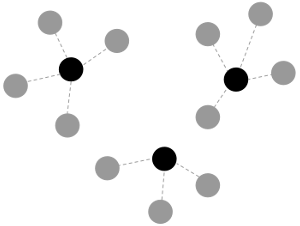
\includegraphics[width=1\textwidth]{pmedian.png}
  \caption{Ilustração do problema da p-Mediana. Na imagem, vemos os centros (círculos)
  sendo atendidos pelas medianas (centros em preto). A relação de atendimento entre um centro
  e uma mediana é representada pelas linhas tracejadas.}
  \label{fig:pmedian}
\end{figure}

\section{MODELAGEM} \label{sec:model}

Para utilizar o Algoritmo de Colônia de Formiga para o problema da p-Mediana, é necessário realizar uma
modelagem relativa à construção de soluções, comportamento de formigas, depósito de feromônio, entre outros
aspectos. No trabalho em questão, a modelagem seguiu em grande parte \cite{dblp:fr}.

Mais formalmente, podemos definir o problema da seguinte forma:

\begin{enumerate}
 \item Seja \textbf{n} o número de centros.
 \item Seja \textbf{p} o número de medianas a serem selecionadas.
 \item Seja $ a_i $ a demanda do centro $ i $.
 \item Seja $ c_j $ a capacidade da mediana $ j $.
 
 \item Seja \textbf{d} a matriz de dimensão $ n $ x $ n $ onde $ d_{ij} $ representa a distância entre
 os centros $ i $ e $ j $.
 
 \item Seja \textbf{x} a matriz de dimensão $ n $ x $ n $ onde $ x_{ij} = 1 $ se o centro $ i $ é atendido
 pela mediana $ j $ e $ 0 $ caso contrário.
 
 \item Dessa forma, o problema da p-Mediana trata-se do problema de minimizar
 $ \sum_{i=1}^{n} \sum_{j=1}^{n} d_{ij}x_{ij} $, considerando algumas restrições:
 
 \begin{enumerate}
  \item $ \sum_{i=1}^{p} x_{ij} = 1, j~=~1,...,p. $
  \item $ \sum_{i=1}^{n} x_{ij}a_i \leq c_j,j~=~1,...,p. $
 \end{enumerate}

\end{enumerate}

\subsection{Algoritmo}

A estrutura geral do Algoritmo de Colônia de Formigas é apresentada na listagem a seguir. Percebemos
que trata-se de um algoritmo simples a alto nível, sendo cada um de seus procedimentos internos variados
de acordo com o problema em questão.\\

\begin{mdframed}[linecolor=black, leftline=false, rightline=false]
    \inputminted[linenos, fontsize=\footnotesize]{text}{pseudo.txt}
\end{mdframed}

\begin{center}
 \textbf{Listagem 1: Pseudocódigo para o Algoritmo de Colônia de Formigas. iter se refere a iteração atual e
 max\_it ao número total de iterações a serem executadas.}
\end{center}

Na Listagem 1, o procedimento \textbf{constrói\_solução()} constrói uma solução para o problema tendo
como base as quantidades de feromônio e outras heurísticas opcionais. Cada formiga passa por um centro
a cada passo de uma iteração. Já o procedimento \textbf{atualiza\_feromônio()} utiliza a informação 
de qualidade de cada solução construída e atualiza as quantidades de feromônio depositadas.

\subsection{Feromônio}

Na implementação desse trabalho, como sugerido em \cite{dblp:fr}, os níveis
de feromônio são referentes aos centros. Dessa forma, um vetor $ \tau $ armazena a quantidade de feromônio
depositada em cada centro.

Dessa forma, durante a etapa de construção de soluções, as formigas escolhem probabilisticamente os centros
que servirão de mediana com base na quantidade de feromônio presente em cada um. Como decisão de implementação,
os níveis de feromônio só são atualizados por formigas que geraram soluções ótimas locais ou globais. A fórmula
que determina como é feita a atualização dos níveis de feromônio com base em uma solução $ S $ é:

\begin{displaymath}
 \tau_i = \rho * \tau_i + \Delta\tau_i
\end{displaymath}

Onde $ \rho $ representa a taxa de evaporação do feromônio $ \tau_i $ já presente em um centro $ i $ e
$ \Delta\tau_i $ é dado por:

\begin{displaymath}
 \Delta\tau_i = \frac{1}{f(S)} 
\end{displaymath}

se $ i \in S $, $ 0 $ caso contrário. $ f(S) $ é uma função que retorna a qualidade da solução $ S $.
Para isso, o custo da solução $ S $ é normalizado no intervalo entre o custo da melhor solução encontrada
até o momento e o custo da pior, sendo o primeiro equivalente a $ 1 $ e o segundo a $ 0 $.

\subsection{Construção de Soluções}

Para construir soluções, as formigas consideram o nível de feromônio presente nos centros. Com esses níveis,
existe uma probabilidade associada à escolha de cada centro pelas formigas, que escolhem os $ p $ centros
que serão medianas um por um, considerando a probabilidade dada por:

\begin{displaymath}
 p_i^k(t) = \frac{\tau_i(t)^\alpha * \eta_i ^ \beta}{\sum_{i \in J^k}^{} \tau_i(t)^\alpha * \eta_i^\beta}
\end{displaymath}

se $ i \in J^k $, onde $ J^k $ é a lista de centros ainda não escolhidos pela formiga $ k $, $ \eta_i $
é uma função heurística descrita na Seção \ref{sec:infheur} e $ \alpha $ e $ \beta $ são parâmetros de peso
do feromônio e da heurística, definidos pelo usuário. Caso $ i \notin J^k $, $ p_i^k(t) = 0 $.

Após a seleção de $ p $ centros para serem medianas, cada um dos $ n - p $ centros restantes devem ser alocados
a precisamente uma mediana. Para isso, uma heurística definida em \cite{dblp:fr}
é utilizada, sendo uma instância do Problema de Alocação Generalizada (tradução livre de Generalized Assignment
Problem - GAP). O Pseudocódigo que descreve a heurística é apresentado na Listagem 2.\\

\begin{mdframed}[linecolor=black, leftline=false, rightline=false]
    \inputminted[linenos, fontsize=\footnotesize]{text}{gap.txt}
\end{mdframed}

\begin{center}
 \textbf{Listagem 2: Pseudocódigo para a heurística do GAP. O procedimento centros\_ordenados() gera uma lista
 com todos os n centros em ordem crescente de distância a suas correspondentes medianas mais próximas. O procedimento
 ordena\_medianas() gera uma lista com todas as p medianas em ordem crescente de distância ao centro passado
 como parâmetro. Importante notar que à medida que os centros vão sendo alocados às medianas, a capacidade das mesmas
 vai diminuindo. Além disso, uma vez que um centro é alocado, o algoritmo sai do loop mais interno.}
\end{center}

\subsection{Heurística de Informação} \label{sec:infheur}

Para melhorar as soluções construídas pelas formigas, \cite{dblp:fr} sugere
a implementação de uma heurística que considera a qualidade da escolha de cada centro como parte da solução.

Nessa heurística, a informação de distância entre o centro sendo analisado e o restante é necessária. Aqui,
a ideia é calcular a densidade otimista dos centros se um dado centro fosse escolhido como mediana. O algoritmo
da heurística é mostrado na Listagem 2.\\

\begin{mdframed}[linecolor=black, leftline=false, rightline=false]
    \inputminted[linenos, fontsize=\footnotesize]{text}{infheur.txt}
\end{mdframed}

\begin{center}
 \textbf{Listagem 3: Pseudocódigo para a Heurística de Informação implementada. O procedimento
 ordena\_centros(centro) ordena todos os centros com base na distância entre eles e o centro passado
 como parâmetro. O procedimento aloca(centro, centros\_ordenados) associa cada centro em centros\_ordenados
 ao centro passado como parâmetro, até que sua capacidade seja atingida, retornando dois valores: (i) todos\_centros:
 o número de centros alocados com sucesso; e (ii) soma\_distância: a soma de todas as distâncias entre os centros
 alocados e o centro passado como parâmetro.}
\end{center}

\section{IMPLEMENTAÇÃO}

Seguindo a modelagem do problema mostrada na Seção \ref{sec:model}, o programa foi implementado
utilizando a linguagem Python 3\footnote{https://www.python.org/download/releases/3.0/}. O programa
utiliza intensivamente a módulo NumPy\footnote{http://www.numpy.org/} da linguagem,
principalmente para a geração de números aleatórios. As classes desenvolvidas
e a estrutura do código fonte são apresentadas a seguir.

\begin{itemize}
 \item Classe \textbf{Client}, arquivo client.py. Define um centro presente no espaço. Para isso,
 armazena as informações de coordenadas, demanda e capacidade (para centros escolhidos como medianas).
 
 \item Arquivo \textbf{tp2.py}. Define o programa principal com os parâmetros de linha de comando e
 entrada e saída.
 
 \item Classe \textbf{ACO}, arquivo aco.py. Define uma instância do problema de p-Mediana como otimização
 por colônia de formigas. Armazena todas as informações como número de centros, medianas, vetor de feromônio,
 valores máximos e mínimos para feromônio, melhor solução global, etc.
\end{itemize}

Algumas decisões de implementação importantes são apresentadas a seguir:

\begin{itemize}
 \item A fim de evitar que os valores de feromônio tendam a se tornarem arbitrariamente grandes 
 (ou pequenos), foram definidos valores de feromônio mínimo e máximo. O valor mínimo é $ 0.001 $
 e o máximo é $ 0.999 $.
 
 \item O valor inicial de feromônio presente em todos os centros é definido como $ 0.5 $, seguindo
 \cite{dblp:fr}.
 
 \item Uma política para evitar que o algoritmo fique estagnado é implementada, também tendo como 
 referência o que é feito em \cite{dblp:fr}. Para isso, uma fórmula
 que depende do valor máximo de feromônio, número de medianas, número de centros e valor mínimo de
 feromônio é utilizada. Quando a soma do valores de feromônio presentes no vetor de feromônio atinge
 o valor retornado pela fórmula, o vetor de feromônio é reinicializado.
 
 \item Somente formigas que geram ótimos locais ou globais atualizam o vetor de feromônio.
 
\end{itemize}

\section{ESTRUTURA DO PROJETO E EXECUÇÃO}

Os arquivos de código-fonte do projeto se encontram na pasta \textbf{src}. 

\subsection{Parâmetros}

A fim de facilitar a execução do programa, foram definidos parâmetros para alterar 
alguns pontos chave para Programação Dinâmica. São eles:

\begin{itemize}
 \item \textbf{Arquivo de entrada:} Arquivo com os dados de entrada a serem usados pelo programa.
 
 \item \textbf{Semente:} Número inteiro usado na geração de números aleatórios durante a 
 execução do programa. Note que, mantendo todos os outros parâmetros fixos, a saída
 do programa para uma mesma entrada e valor de semente será sempre igual. A semente
 da execução pode ser definida com a flag \textbf{-s} e tem valor padrão $ 0 $.
 
 \item \textbf{Número de formigas:} Número inteiro que determina o número total de formigas
 que serão utilizadas para gerar soluções do problema. Pode ser definido com a flag \textbf{-n}
 e tem valor padrão $ 4 $.
  
 \item \textbf{Número de iterações:} Define o número de iterações pelo qual o programa
 deve executar. Definido com a flag \textbf{-i} e tem valor padrão $ 10 $.
 
 \item \textbf{Taxa de evaporação de feromônio:} Taxa segundo a qual os valores de feromônio
 depositado nos centros desaparecem com o tempo. Definida com a flag \textbf{-d} e tem valor
 padrão $ 0.8 $.
 
 \item \textbf{Peso para feromônio (alpha):} Peso do feromônio no cálculo de probabilidade de escolher 
 um centro. Definido com a flag \textbf{-a} e tem valor padrão $ 3 $.
 
 \item \textbf{Peso para heurística de informação (beta):} Peso da heurística de informação no cálculo
 de probabilidade de escolher um centro. Definido com a flag \textbf{-b} e tem valor padrão $ 1 $.
\end{itemize}

Para executar o programa, o comando abaixo é usado:

\begin{center}
tp2.py [-h] [-n ANTN] [-i MAXIT] [-d DECAYR] [-a ALPHA] [-b BETA]
              [-s RSEED]
              INPUT\_FILE
\end{center}

Onde RSEED indica a semente, ANTN o número de formigas, MXIT o número de iterações do algoritmo,
DECAYR a taxa de evaporação do feromônio, ALPHA e BETA os pesos de feromônio e heurística de informação, 
respectivamente), INPUT\_FILE o nome do arquivo de entrada.

Todos os parâmetros entre colchetes acima são opcionais.

\subsection{Entrada e Saída}

Os arquivos de entrada devem possuir a mesma estrutura. Neles, a primeira linha deve conter
os valores de $ n $ e $ p $, separados por um espaço. Nas $ n $ linhas seguintes, são listados
os dados dos centros, i.e., $ x $, $ y $, $ c $ e $ d $, que são a coordenada $ x $, coordenada
$ y $, capacidade $ c $ do centro e demanda $ d $, respectivamente.

Em relação à saída do programa, é impresso, a cada iteração, o número da mesma e os valores
de melhor solução global e local. Ao final é impresso o custo da melhor solução achada para o
programa.

\section{EXPERIMENTOS}

Nessa seção serão apresentados os experimentos realizados. Todos eles foram executados em
uma máquina Intel Core i7-5500U, 2.40GHz, 4 cores, 8GB de memória RAM e sistema operacional
ubuntu 14.04 LTS.

\subsection{Metodologia}

Muitas instâncias de teste foram executadas para cada uma das bases de teste. A metodologia
utilizada foi um processo iterativo de determinação de parâmetros ótimos para cada um dos
três arquivos de entrada fornecidos com o trabalho. A cada etapa, um dos parâmetros era o 
foco do experimento, que procurava identificar configurações ótimas ou próximas disso.

Uma vez determinados esses parâmetros ótimos, seguia-se para o próximo parâmetro a determinar,
fixando-se aqueles já determinados anteriormente.

\subsection{Experimentos}

Abaixo são mostrados os principais experimentos realizados. Os resultados são apresentados
na Seção \ref{sec:result}. Os valores apresentados foram obtidos da média de 30 execuções.

\begin{itemize}
 \item \textbf{Experimento 1:} No primeiro experimento, objetivou-se simplesmente a verificação
 de qual número de formigas utilizado é mais interessante para cada arquivo de teste. Para os
 três, os parâmetros de execução foram:
 
 Número de formigas: [10, 30, 60, 90] \\
 Número de iterações: 50 \\
 Taxa de evaporação: 0.8 \\
 Alpha: 3 \\
 Beta: 1
 
 \item \textbf{Experimento 2:} Nesse segundo experimento, o objetivo foi verificar por quantas
 iterações o programa deveria ser executado par cada arquivo de teste. Os parâmetros utilizados
 para a execução foram os seguintes:
 
 Número de formigas: Definido em Experimento 1. \\
 Número de iterações: 100 \\
 Taxa de evaporação: 0.8 \\
 Alpha: 3 \\
 Beta: 1
 
 \item \textbf{Experimento 3:} O próximo passo foi determinar a taxa de evaporação de feromônio
 ideal para os arquivos de teste. Dessa forma, o programa foi executado para cada um
 dos arquivos com a seguinte configuração:
 
 Número de formigas: Definido em Experimento 1. \\
 Número de iterações: Definido em Experimento 2. \\
 Taxa de evaporação: [0.3, 0.6, 0.8, 0.9] \\
 Alpha: 3 \\
 Beta: 1
 
 \item \textbf{Experimento 4:} Finalmente, tentamos determinar os parâmetros $\alpha$ e $\beta$
 (ver Seção \ref{sec:infheur}). Para isso, três configurações são propostas, uma que prioriza $\alpha$,
 outra que prioriza $\beta$ e outra que dá pesos iguais para os dois parâmetros.
 
 Número de formigas: Definido em Experimento 1. \\
 Número de iterações: Definido em Experimento 2. \\
 Taxa de evaporação: Definido em Experimento 3. \\
 (Alpha, Beta): [(1, 3), (2, 2), (3, 1)]
 
\end{itemize}

\section{RESULTADOS} \label{sec:result}

\subsection{Experimento 1: Número de formigas}

Com esse experimento, conseguimos determinar o número de formigas mais apropriado para cada arquivo
de teste. Mais apropriado aqui refere-se ao valor do parâmetro que mais compensa o custo de tempo e 
resultado obtido. Vemos por exemplo que, para o arquivo SJC1.dat, a variação no número de formigas
causou também uma grande variação no resultado obtido, sendo, portanto, melhor o uso de 90 formigas.

\begin{figure}[!htbp]
  \centering
  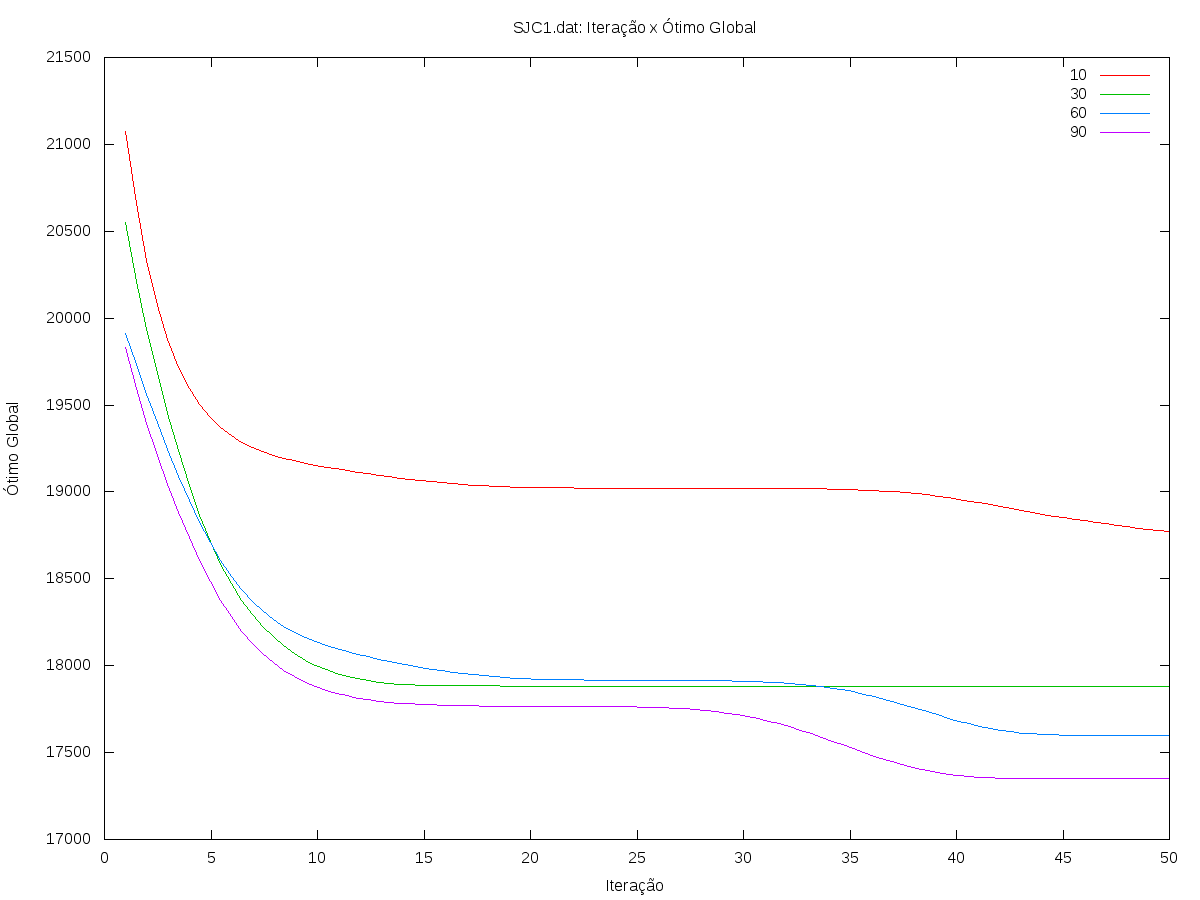
\includegraphics[width=1\textwidth]{exp1s1.png}
  \caption{Experimento 1 - SJC1.dat: Número de iterações x Ótimo global para quantidades variáveis
  de formigas. Cada cor representa uma quantidade de formigas utilizada.}
  \label{fig:exp1s1}
\end{figure}

Para o arquivo SJC2.dat, vemos que os valores de 60 e 90 formigas alcançam resultados muito similares,
não sendo justificável o uso de 90 formigas, que acarreta em perda de desempenho.

\begin{figure}[!htbp]
  \centering
  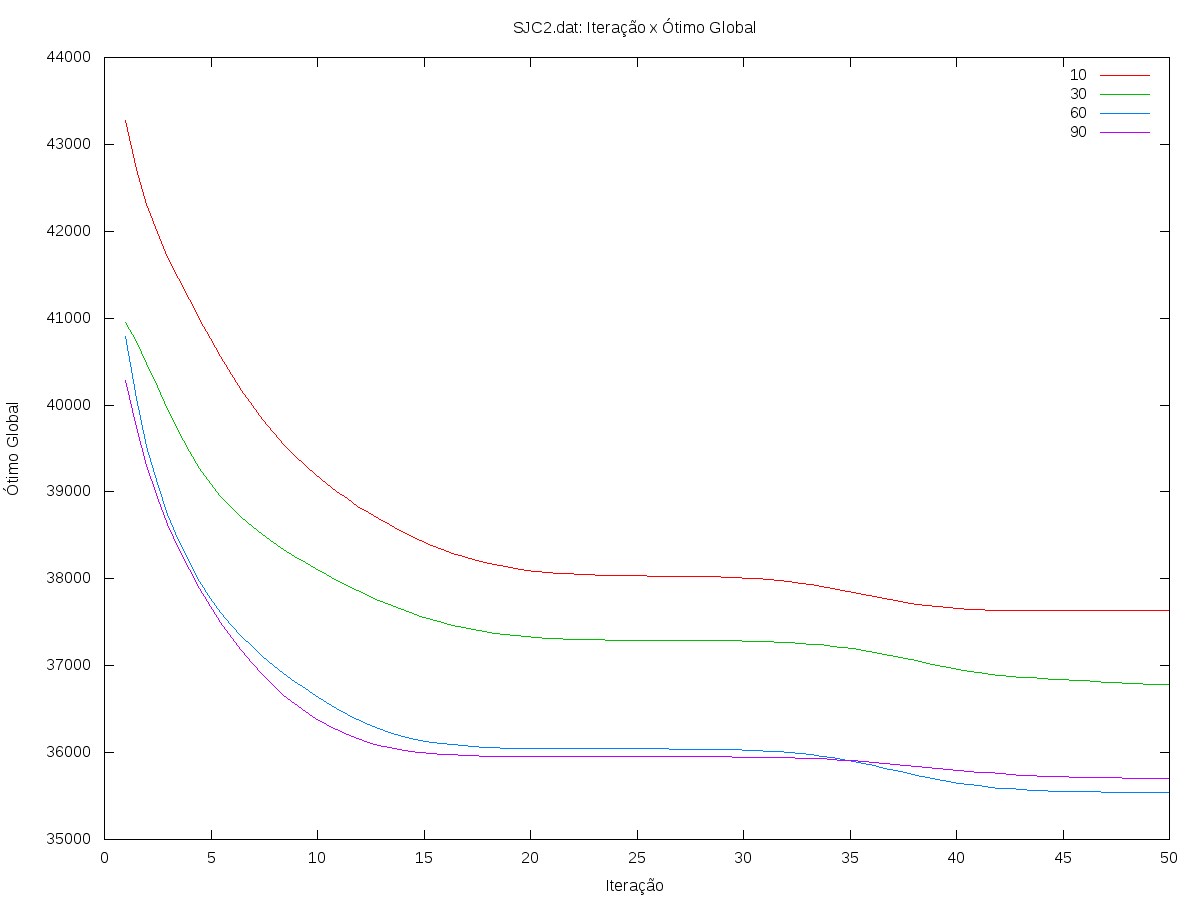
\includegraphics[width=1\textwidth]{exp1s2.png}
  \caption{Experimento 1 - SJC2.dat: Número de iterações x Ótimo global para quantidades variáveis
  de formigas. Cada cor representa uma quantidade de formigas utilizada.}
  \label{fig:exp1s2}
\end{figure}

Finalmente, para o arquivo SJC3.dat, os resultados obtidos para 30. 60 e 90 formigas são muito próximos,
logo, para melhor desempenho em tempo, escolhemos o valor de 30 formigas.

\begin{figure}[!htbp]
  \centering
  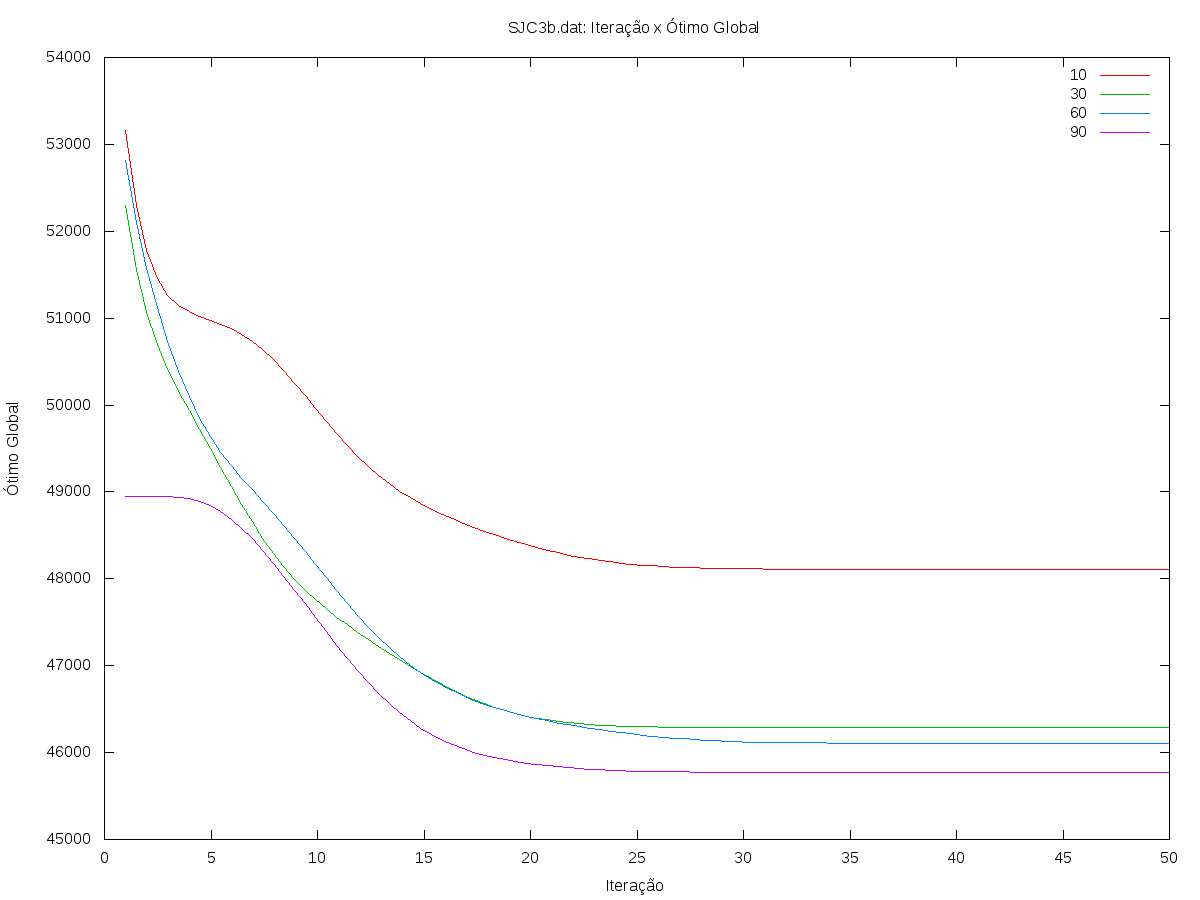
\includegraphics[width=1\textwidth]{exp1s3.png}
  \caption{Experimento 1 - SJC3b.dat: Número de iterações x Ótimo global para quantidades variáveis
  de formigas. Cada cor representa uma quantidade de formigas utilizada.}
  \label{fig:exp1s3}
\end{figure}

As Figuras de \ref{fig:exp1s1} a \ref{fig:exp1s3} mostram os resultados do Experimento 1.

\subsection{Experimento 2: Iterações}

Uma vez definido o número de formigas a ser utilizado para cada um dos arquivos teste, é necessário
determinar por quantas iterações o programa deve executar para cada arquivo, uma vez que valores próximos
do ótimo podem ser encontrados em uma iteração $ i $, não sendo necessário executar o programa por mais
que $ i $ iterações.

Podemos ver na Figura \ref{fig:exp2s1} que para o arquivo de entrada SJC1.dat, o algoritmo não
consegue melhor a solução após meados de 50 iterações. O mesmo acontece para os arquivos
SJC2.dat e SJC3b.dat com os valores de 25 e 30 iterações, respectivamente, como visto nas
Figuras \ref{fig:exp2s2} e \ref{fig:exp2s3}. Logo, não
precisamos rodar o programa para valores de iterações acima desses valores.

\begin{figure}[!htbp]
  \centering
  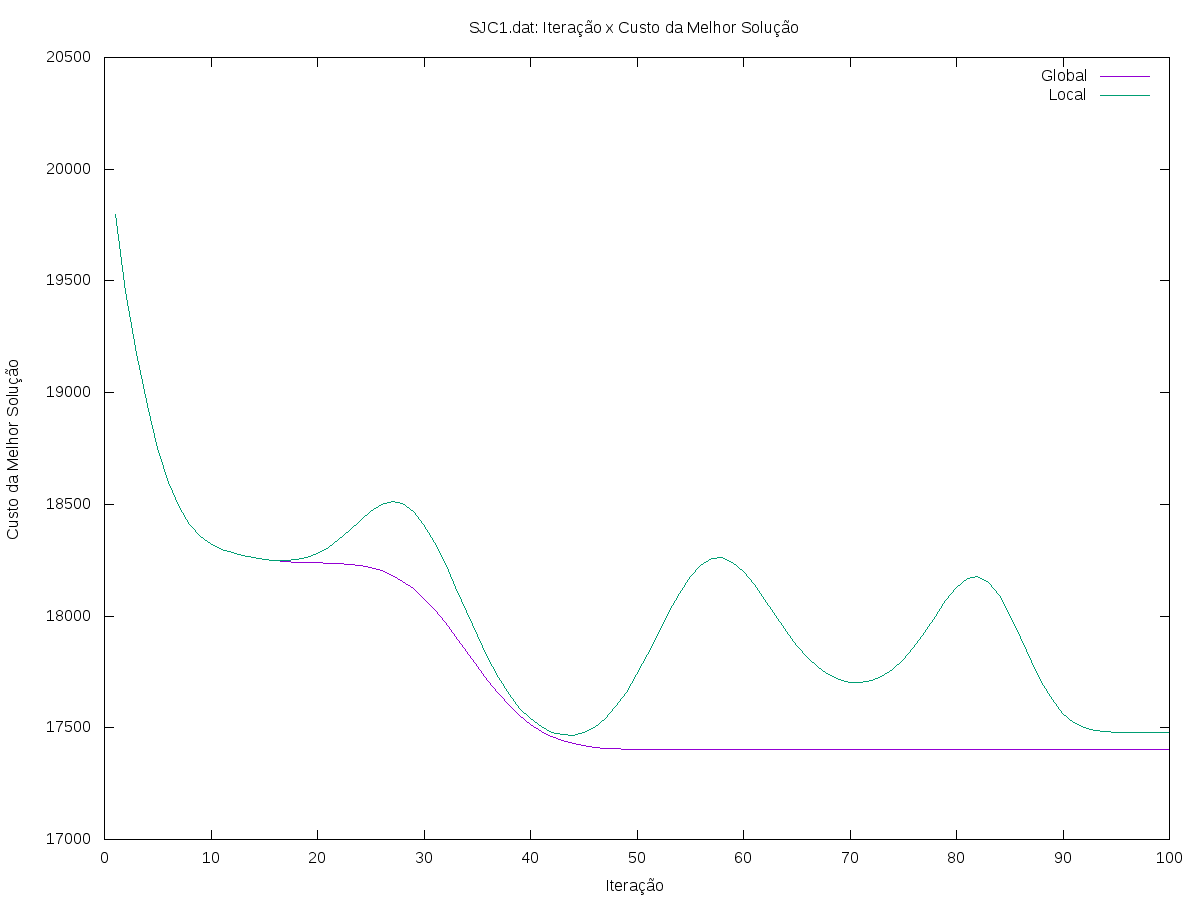
\includegraphics[width=1\textwidth]{exp2s1.png}
  \caption{Experimento 2 - SJC1.dat: Número de iterações x Custo da melhor solução global e local.}
  \label{fig:exp2s1}
\end{figure}

\begin{figure}[!htbp]
  \centering
  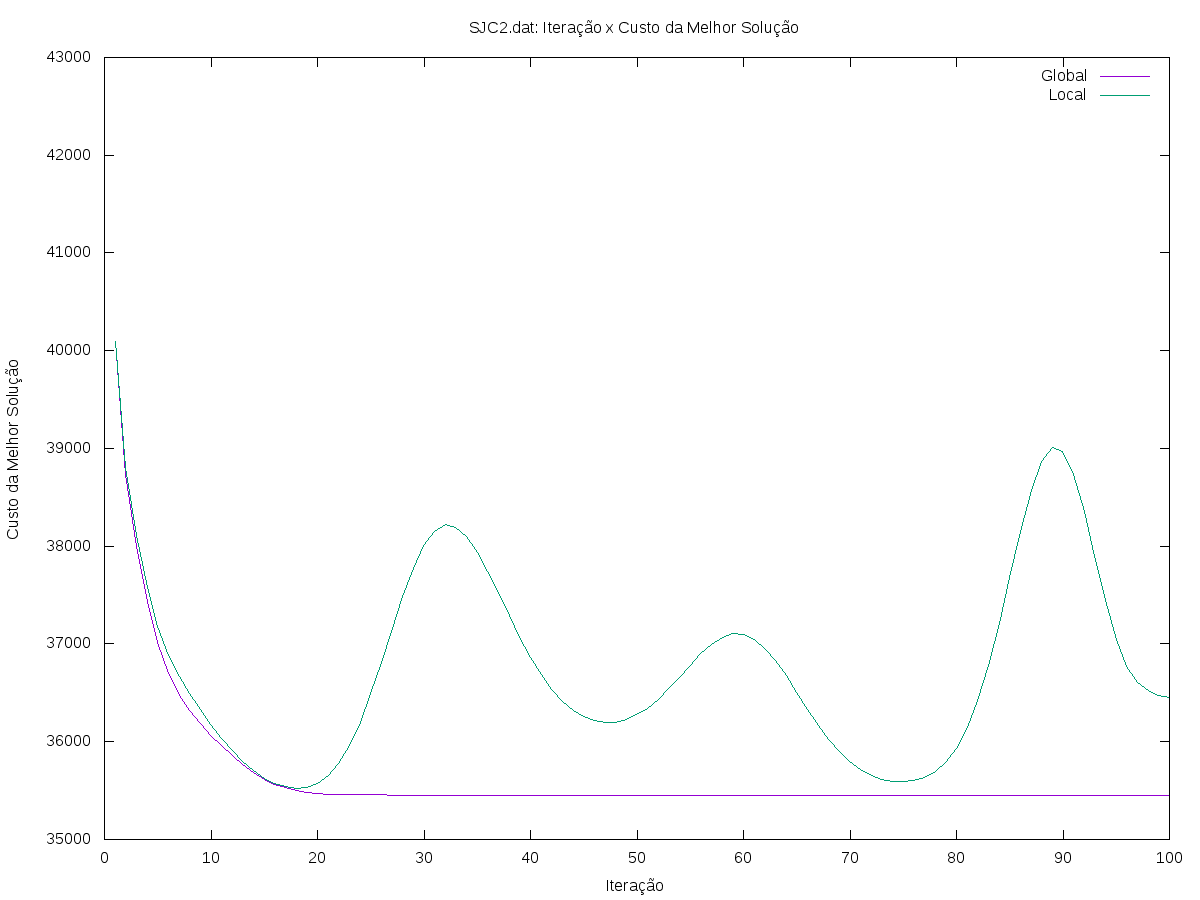
\includegraphics[width=1\textwidth]{exp2s2.png}
  \caption{Experimento 2 - SJC2.dat: Número de iterações x Custo da melhor solução global e local.}
  \label{fig:exp2s2}
\end{figure}

\begin{figure}[!htbp]
  \centering
  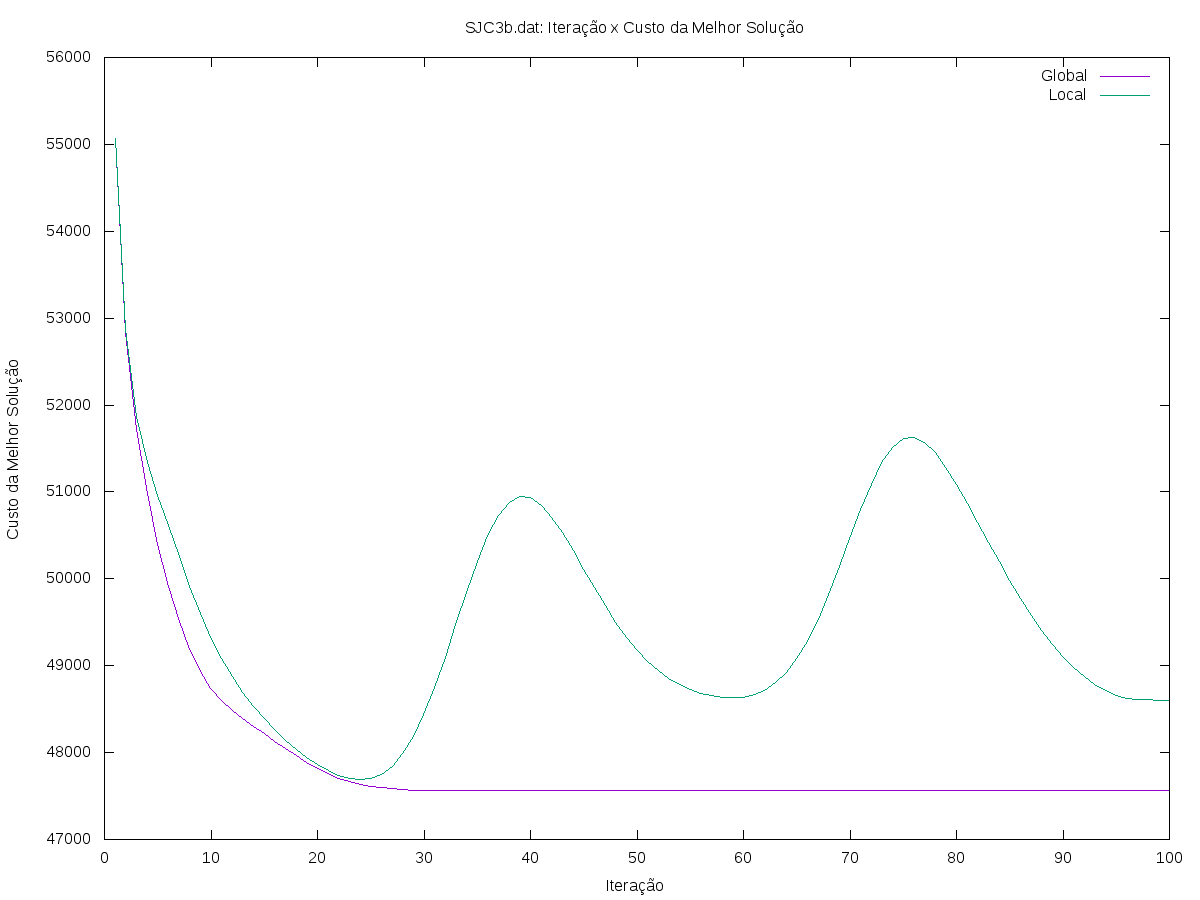
\includegraphics[width=1\textwidth]{exp2s3.png}
  \caption{Experimento 2 - SJC3b.dat: Número de iterações x Custo da melhor solução global e local.}
  \label{fig:exp2s3}
\end{figure}

\subsection{Experimento 3: Taxa de Evaporação}

Continuando com o processo iterativo de determinação dos parâmetros ótimos, precisamos determinar a taxa de
evaporação de feromônio depositado nos centros. Para isso, foram propostos quadro valores para esse parâmetro,
um muito baixo, outro médio e dois altos ($0.3$, $0.6$, $0.8$ e $0.9$). Podemos ver nas Figuras de \ref{fig:exp3s1}
a \ref{fig:exp3s3} que, para todos os arquivos teste, a taxa de evaporação de feromônio com melhores resultados
é $ 0.8 $.

\begin{figure}[!htbp]
  \centering
  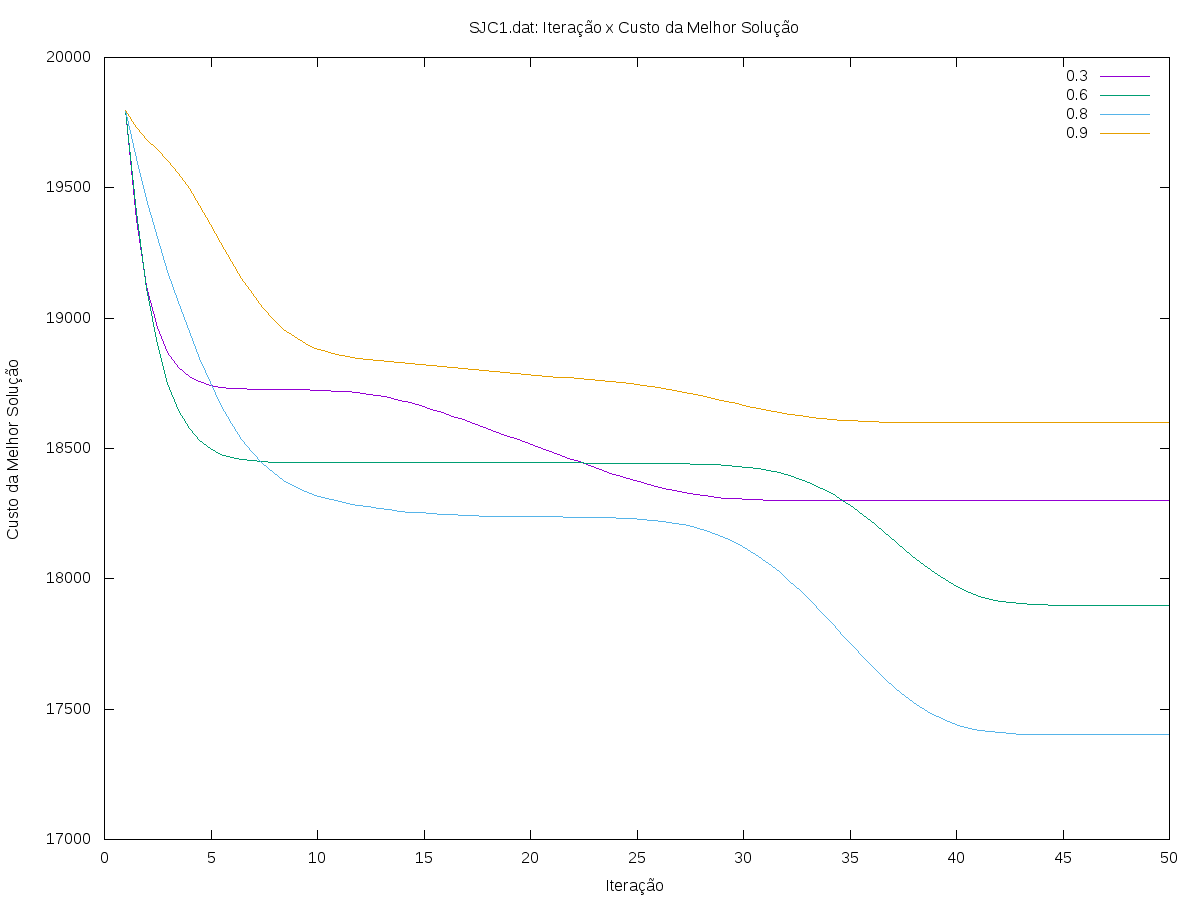
\includegraphics[width=1\textwidth]{exp3s1.png}
  \caption{Experimento 3 - SJC1.dat: Número de iterações x Custo da melhor solução com taxas
  de evaporação de feromônio variáveis.}
  \label{fig:exp3s1}
\end{figure}

\begin{figure}[!htbp]
  \centering
  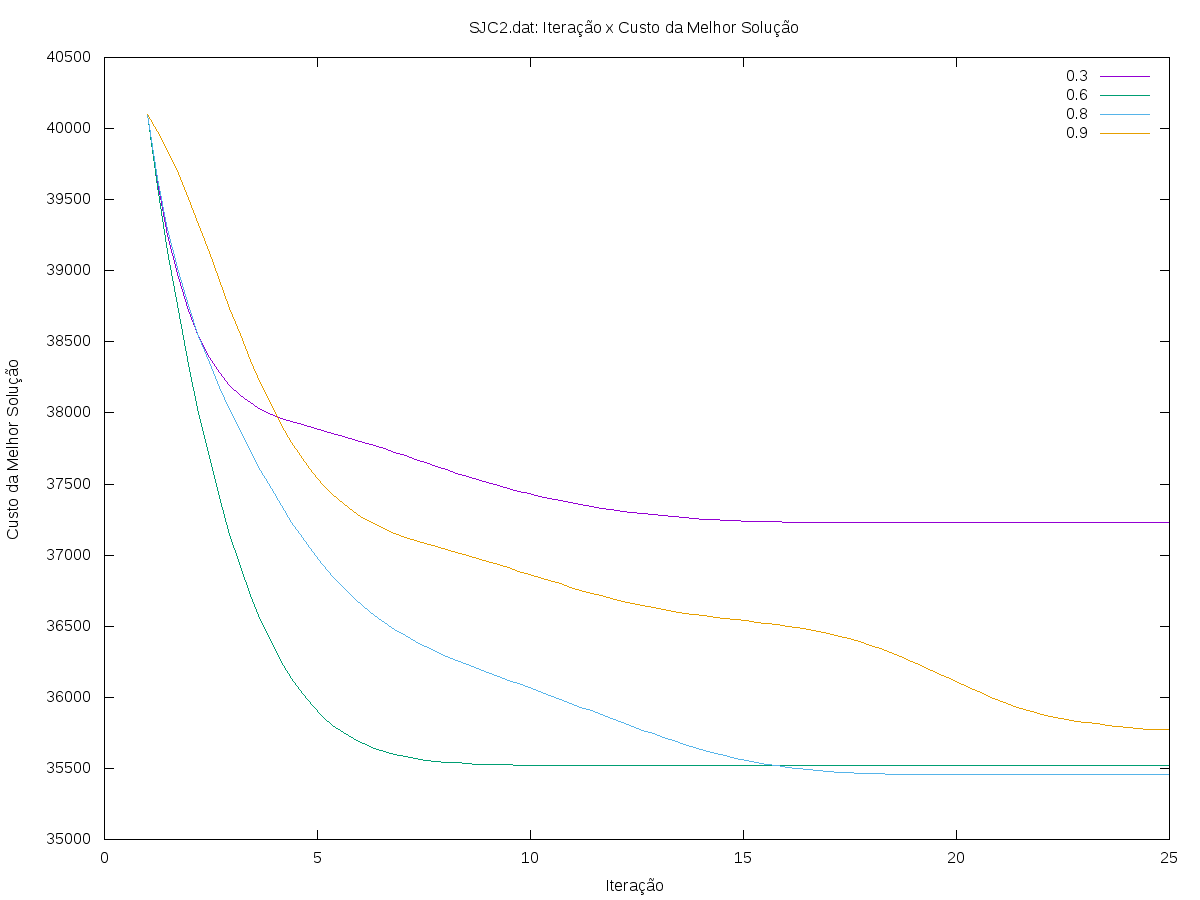
\includegraphics[width=1\textwidth]{exp3s2.png}
  \caption{Experimento 3 - SJC2.dat: Número de iterações x Custo da melhor solução com taxas
  de evaporação de feromônio variáveis.}
  \label{fig:exp3s2}
\end{figure}

\begin{figure}[!htbp]
  \centering
  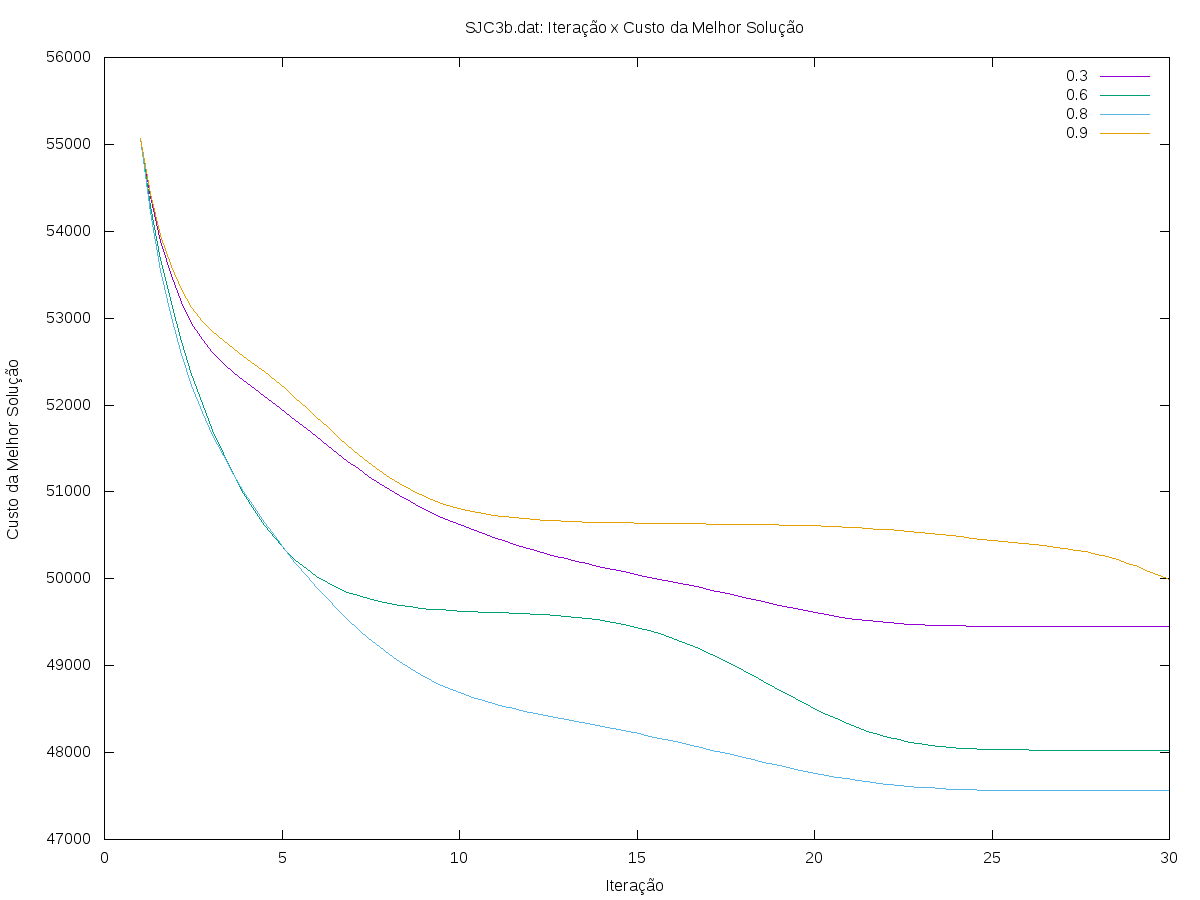
\includegraphics[width=1\textwidth]{exp3s3.png}
  \caption{Experimento 3 - SJC3b.dat: Número de iterações x Custo da melhor solução com taxas
  de evaporação de feromônio variáveis.}
  \label{fig:exp3s3}
\end{figure}

\subsection{Experimento 4: $\alpha$ e $\beta$}

Com o Experimento 4, cujos resultados são ilustrados nas Figuras de \ref{fig:exp4s1} a \ref{exp4s3}, vemos
que esses parâmetros são muito relativos ao arquivo de entrada utilizado, uma vez que para SCJ1.dat e SJC2.dat
a melhor configuração foi $\alpha = 2, \beta = 2$ e para SJC3b.dat foi $\alpha = 3, \beta = 1$.

\begin{figure}[!htbp]
  \centering
  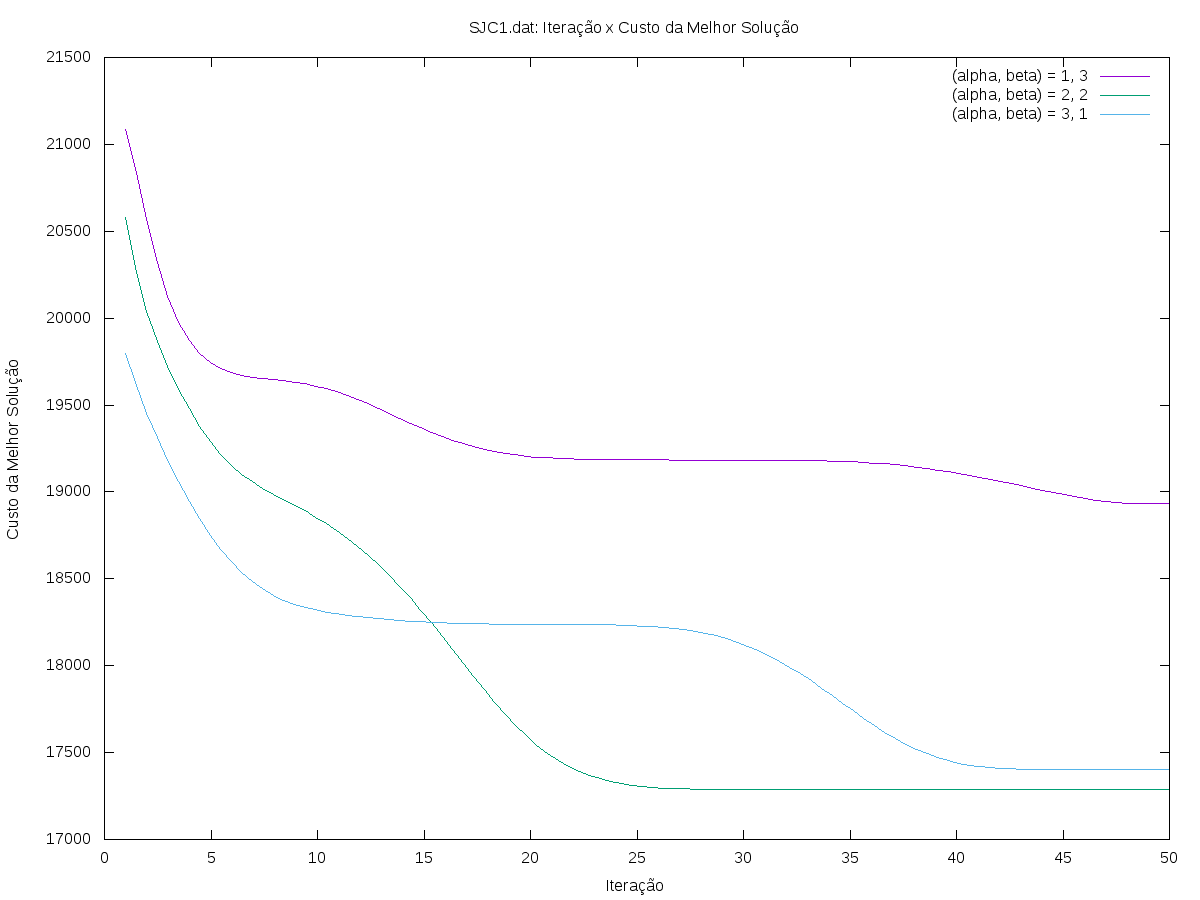
\includegraphics[width=1\textwidth]{exp4s1.png}
  \caption{Experimento 4 - SJC1.dat: Número de iterações x Custo da melhor solução com parâmetros $\alpha$ 
  e $\beta$ variáveis.}
  \label{fig:exp4s1}
\end{figure}

\begin{figure}[!htbp]
  \centering
  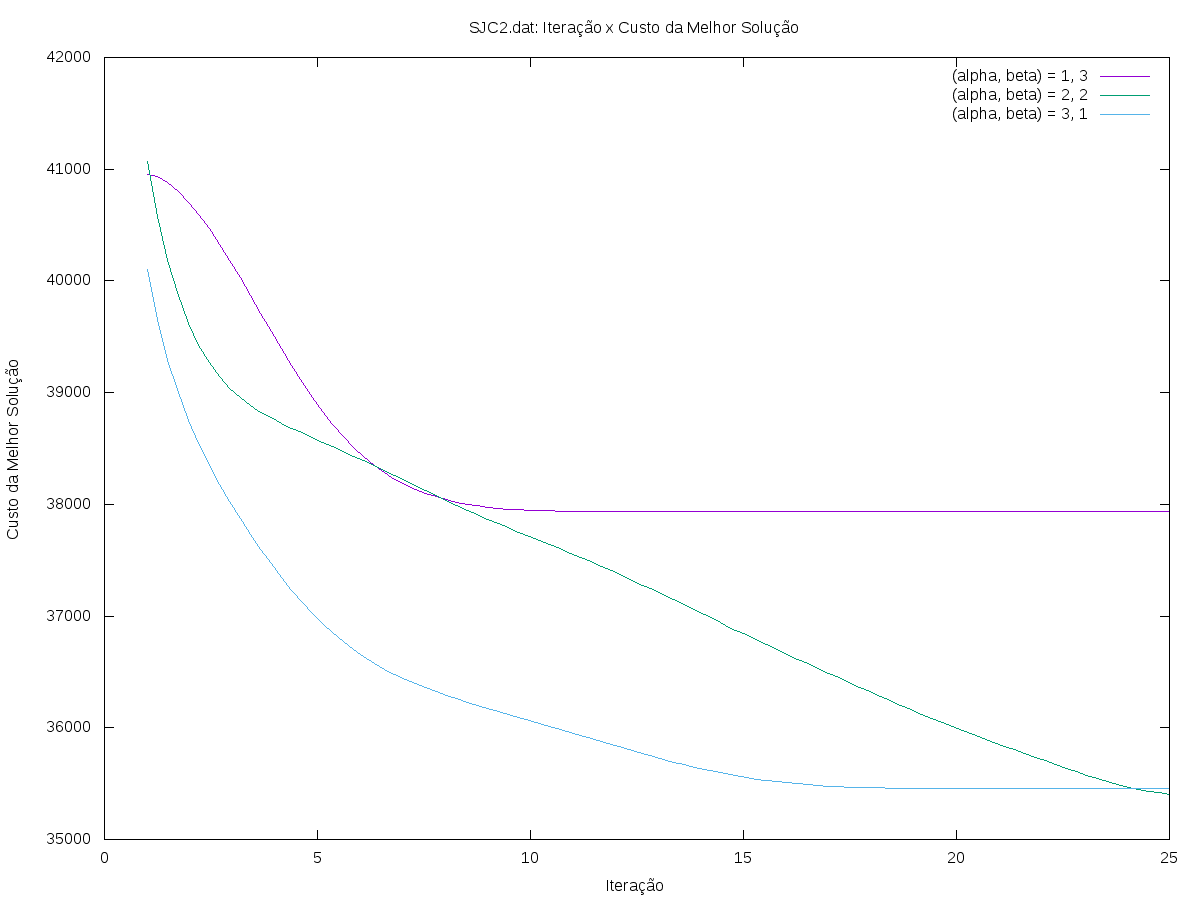
\includegraphics[width=1\textwidth]{exp4s2.png}
  \caption{Experimento 4 - SJC2.dat: Número de iterações x Custo da melhor solução com parâmetros $\alpha$ 
  e $\beta$ variáveis.}
  \label{fig:exp4s2}
\end{figure}

\begin{figure}[!htbp]
  \centering
  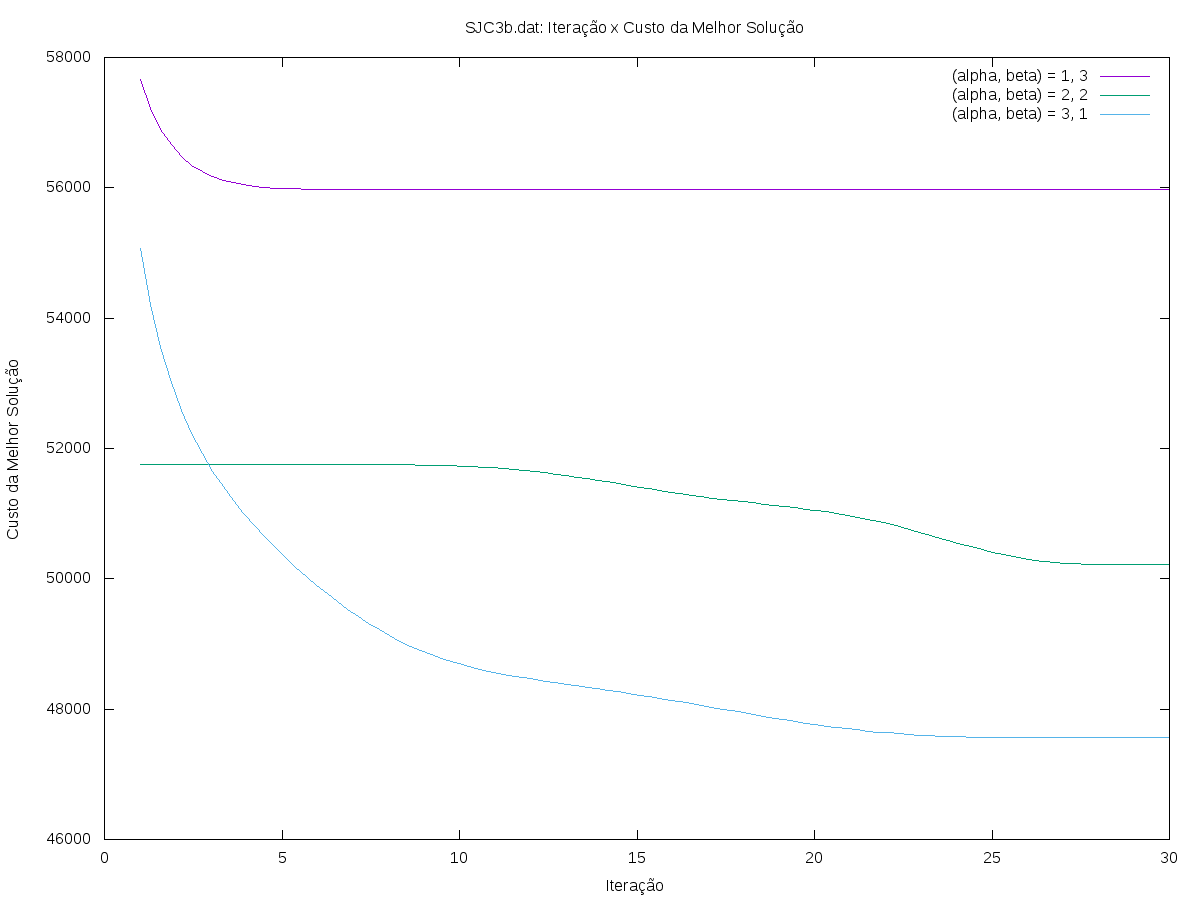
\includegraphics[width=1\textwidth]{exp4s3.png}
  \caption{Experimento 4 - SJC3b.dat: Número de iterações x Custo da melhor solução com parâmetros $\alpha$ 
  e $\beta$ variáveis.}
  \label{fig:exp4s3}
\end{figure}

\subsection{Análise}

Os experimentos realizados possibilitaram observar diversas características importantes, tanto
de otimização por colônia de formigas em geral quanto a respeito dos arquivos de entrada utilizados.
Vimos aqui que a escolha do número de formigas, por exemplo, determina o nível de exploração
do espaço de busca. Sendo cada uma das formigas responsável por seguir por um 'caminho' ao procurar
soluções para o problema.

Importante notar que o trabalho seguiu o que foi feito em \cite{dblp:fr},
sendo assim, interessante em trabalhos relacionados que utilizem o algoritmo de colônia de formigas a
utilização de outros trabalhos de referência, para fins de comparação em algum projeto futuro.

\begin{center}
 \begin{tabular}{|c|c|c|c|c|} \hline
 Arquivo & Nós & P & Ótimo & Obtido \\ \hline
 SJC1.dat & $ 100 $ & $ 10 $ & $ 17246,53 $ & $ 17287,54 $ \\ \hline
 SJC2.dat & $ 200 $ & $ 15 $ & $ 33225,88 $ & $ 35401,82 $ \\ \hline
 SJC3b.dat & $ 300 $ & $ 30 $ & $ 40635,80 $ & $ 47561,58 $ \\ \hline
 \end{tabular} 
\end{center}

\section{CONCLUSÃO}

Com esse trabalho, os conceitos fundamentais de Otimização por Colônia de Formigas puderam ser
fixados. A estrutura geral do algoritmo é muito simples e podemos perceber que os detalhes de
implementação na verdade são muito dependentes do problema a ser resolvido. Também é importante
notar que a modelagem do problema, mais uma vez, exerce papel fundamental tanto na performance
quanto em complexidade de código e outros fatores.

Assim como no trabalho prático 1, a maior dificuldade foi a de lidar com o tempo demandado pela
execução de experimentos. Cada instância do algoritmo, isto é, configuração de parâmetros a ser
executada demora uma quantidade muito grande de tempo.

De maneira geral vemos que os valores de custo obtidos ao final do trabalho são muito bons quando
comparados com os valores de ótimo fornecidos com as bases de teste. Logo, o algoritmo de colônia 
de formigas é realmente muito competitivo, principalmente tendo em mente que o problema da 
p-Mediana é NP-difícil.

\section{REFERÊNCIAS}

\bibliographystyle{sbc}
\bibliography{sbc-template}

\end{document}
